\documentclass[addpoints,11pt]{exam}

\usepackage{alltt}
\usepackage[margin=1in]{geometry}   % set up margins
\usepackage[T1]{fontenc}
\usepackage[usenames,dvipsnames]{xcolor}
\usepackage{enumerate}              % fancy enumerate
\usepackage{amsmath}                % used for \eqref{} in this document
\usepackage{amsthm}
\theoremstyle{definition}
\newtheorem{exmp}{Example}[section]
\usepackage{verbatim}               % useful for \begin{comment} and \end{comment}
\usepackage{eurosym}                % used for euro symbol
\usepackage{caption} 
\usepackage{graphicx}
\graphicspath{{Figures/}}
\usepackage{subcaption}
\usepackage{color}
\usepackage{float}
\usepackage{amssymb}
\usepackage{sgamevar}
\usepackage{sgame}
\usepackage[colorlinks=true]{hyperref}
\hypersetup{colorlinks=true, citecolor=ForestGreen, linkcolor=BlueViolet, urlcolor=Magenta}



%Solutions or nah (blank next two lines out for no solutions, unblank #3)
%\printanswers
%\newcommand{\dd}[1]{\par {\textbf{\textcolor{red}{#1}}}}
\newcommand{\dd}[1]{}  


\setlength\parindent{0pt}
\unframedsolutions
\SolutionEmphasis{\color{red}}
\CorrectChoiceEmphasis{\color{red}}
\renewcommand{\choicelabel}{(\alph{choice})}
\newcommand{\blank}[0]{\underline{\hspace{3cm}}}
\pointformat{\bfseries[\thepoints]}
\pointpoints{pt}{pts}
\pointsinrightmargin


\begin{document}
	
	

\title{\textbf{Problem Set 6 \dd{Answers and Selected Solutions}} \\ \vspace{2 mm} {\large Principles of Economics}}
\author{David A. D\'iaz}
\date{}
\maketitle

\subsection*{The Monetary System}

\begin{questions}	
	
	\question While cleaning your apartment, you look under the sofa cushion and find a \$50 bill. You deposit the bill in your checking account. The Fed's reserve requirement is 20\% of deposits. What is the maximum amount that the money supply could increase?
	
	\begin{choices}
		\choice \$10
		\choice \$50
		\CorrectChoice \$200
		\choice \$250
	\end{choices}
	
	\begin{solution}
		Your deposit will could increase the money supply through the banking system by $50 \times 1/.20 = \$250$, but you removed \$50 in currency and so the maximum increase in the MS is \$200.
	\end{solution}
	
	
	\question Chloe takes \$100 of currency from her wallet and deposits it in a checking account. If the bank adds the entire \$100 to reserves, the money supply \blank, but if the bank lends out some of the \$100, the money supply \blank.
	
	\begin{choices}
		\choice increases; increases even more
		\choice increases; increases by less
		\CorrectChoice is unchanged; increases
		\choice decreases; decreases by less
	\end{choices}
	
	
	
	\question In a system of fractional-reserve banking, even without any action by the central bank, the money supply declines if households choose to hold \blank currency or if banks choose to hold \blank excess reserves.
	
	\begin{choices}
		\CorrectChoice more; more
		\choice more; less
		\choice less; more
		\choice less; less
	\end{choices}
	
	\begin{solution}
		If people hold more in currency, banks cannot lend out as much money. If banks hold excess reserves, they are not loaning as much money as they could be.
	\end{solution}
	
	\question Suppose an economy contains 2,000 \$1 bills. If people initially deposit half their currency as demand deposits while banks maintain 100\% reserves, the maximum quantity of money would be \blank. If, however, people initially deposit half their currency as demand deposits while banks maintain 10\% reserves, the maximum quantity of money is \blank.
	
	\begin{choices}
		\choice \$2,000; \$10,000
		\choice \$1,000; \$10,000
		\choice \$1,000; \$11,000
		\CorrectChoice \$2,000; \$11,000
	\end{choices}
	
	\begin{solution}
		In a 100\% reserve banking system, the money supply does not change if people hold money in deposits. \$1,000 are in currency, \$1,000 are in deposits. Under a fractional-reserve system, money is created. \$1,000 are in currency, and \$1,000 $\times$ 1/.10 = \$10,000 are potentially created by the banking system.
	\end{solution}
	
\newpage
	
	\question If the Fed wanted to increase the money supply, it could
	
	\begin{choices}
		\CorrectChoice purchase government bonds.
		\choice increase the required reserve ratio.
		\choice increase the discount rate.
		\choice increase the interest rate on reserves.
	\end{choices}
	
	

	
	\question Suppose a shift in the money supply caused the value of money to decrease from $1/4$ to $1/5$. As such, the price level in the economy
	
	\begin{choices}
		\choice decreased 20\%.
		\CorrectChoice increased 25\%.
		\choice increased 20\%.
		\choice decreased 25\%.
	\end{choices}
	
	\begin{solution}
		Value of money = 1/P $\Rightarrow P_0 = 4$, $P_1 = 5$. $\%\Delta P = (5-4)/4 \times 100\% = +25\%$.
	\end{solution}
	
	
	\question Which of the following is NOT a tool the Fed uses to influence the money supply?
	
	\begin{choices}
		\CorrectChoice Raise/lower taxes
		\choice Purchase/sell bonds
		\choice Pay interest on reserves
		\choice Set reserve requirements
		\choice None of the above
	\end{choices}	

\question The M1 money supply is composed of 

\begin{choices}
	\CorrectChoice currency, demand deposits, traveler's checks, and other checkable accounts.
	\choice currency, demand deposits, savings deposits, money market mutual funds, and small time deposits.
	\choice currency, government bonds, gold certificates, and coins.
	\choice currency, NOW accounts, savings accounts, and government bonds.
	\choice none of the above.
\end{choices}

\question Required reserves of banks are a fixed percentage of their

\begin{choices}
	\choice loans.
	\choice assets.
	\CorrectChoice deposits.
	\choice government bonds.
\end{choices}

\question Which of the following Fed actions is likely to increase the money supply?

\begin{choices}
	\CorrectChoice Reducing reserve requirements.
	\choice Selling government bonds.
	\choice Increasing the discount rate.
	\choice All of these will increase the money supply.
\end{choices}

\newpage

\question Suppose Joe changes his \$1,000 demand deposit from Bank A to Bank B. If the reserve requirement is 10\%, what is the potential change in demand deposits as a result of his actions?

\begin{choices}
	\choice \$1,000
	\choice \$10,000
	\CorrectChoice \$0
	\choice \$9,000
\end{choices}

\question If the Fed engages in an open-market purchase while simultaneously raising reserve requirements,

\begin{choices}
	\choice the money supply should rise.
	\choice the money supply should fall.
	\choice the money supply should remain unchanged.
	\CorrectChoice we cannot be certain what will happen to the money supply.
\end{choices}

\question Suppose the Fed purchases a \$1,000 government bond from you. If you deposit the entire \$1,000 in your bank, what is the total potential change in the money supply if reserve requirements are 20\%?

\begin{choices}
	\choice \$1,000
	\choice \$4,000
	\CorrectChoice \$5,000
	\choice \$0
\end{choices}

\question Which of the following is not a function of money?

\begin{choices}
	\choice Unit of account.
	\choice Store of value.
	\CorrectChoice Hedge against inflation.
	\choice Medium of exchange.
\end{choices}

\question The discount rate is 

\begin{choices}
	\choice the interest rate the Fed pays on reserves.
	\CorrectChoice the interest rate the Fed charges on loans to banks.
	\choice the interest rate banks pay on the public's deposits.
	\choice the interest rate the public pays when borrowing from banks.
\end{choices}
	
\end{questions}

\subsection*{Money Growth and Inflation}

\begin{questions}
	
	\question An economy produces one good -- rice. The economy has enough labor, capital, and land to produce 800 bags. The money supply in this economy is \$2,000 and rice sells for \$5/bag. The nominal GDP in the economy is \blank and the velocity of money is \blank.
	
	\begin{choices}
		\CorrectChoice \$4,000; 2
		\choice \$2,000; 2
		\choice \$4,000; 1
		\choice \$2,000; 1
	\end{choices}
	
	\begin{solution}
		Quantity Theory of Money (in levels): $Mv=PY$, where $PY$ = \$5 $\times$ 800 = \$4,000 = nominal GDP. $v$ = 4000/2000 = 2.
	\end{solution}
	
	\question According to the quantity theory of money and the Fisher effect, if the central bank increases the rate of money growth
	
	\begin{choices}
		\CorrectChoice inflation and the nominal rate will both increase. 
		\choice inflation and the real interest rate both increase.
		\choice the nominal interest rate and the real interest rate both increase.
		\choice inflation, the real interest rate, and the nominal interest rate all increase.
	\end{choices}

	\question Suppose the interest rate on a home mortgage was set with the expectation that the price level would decrease by 3\%. If through the course of the loan, the price level actually did not change, who was hurt most?
	
	\begin{choices}
		\choice The mortgage holder
		\CorrectChoice The bank
		\choice Neither was hurt
		\choice Both were hurt equally
	\end{choices}
	
	\begin{solution}
		Actual inflation was greater than expected inflation, so lenders are hurt.
	\end{solution}
	
	\question You put money in an account that advertises a 5\% interest rate. The inflation rate is 3\%, and the tax rate on your returns is 20\%. Your after-tax nominal rate of interest is \blank and your after-tax real rate of interest is \blank.
	
	\begin{choices}
		\choice 1\%; 2\%
		\choice 1\%; .8\%
		\CorrectChoice 4\%; 1\%
		\choice 4\%; .8\%
	\end{choices}
	
	\begin{solution}
		After-tax nominal rate = 5\% $\times$ (1-.20) = 4\%. After-tax real rate = 4\% - 3\% = 1\%.
	\end{solution}
	
	\question According to the quantity theory of money, an increase in the money supply will cause the price level to 
	
	\begin{choices}
		\choice remain relatively constant since money is neutral.
		\CorrectChoice increase by the same percentage as the money supply.
		\choice increase by a greater percentage than the money supply.
		\choice increase by a smaller percentage than the money supply.
	\end{choices}
	
	\question Suppose a shift in the money supply caused the value of money to decrease from $1/4$ to $1/5$. As such, the price level in the economy
	
	\begin{choices}
		\choice decreased 20\%.
		\CorrectChoice increased 25\%.
		\choice increased 20\%.
		\choice decreased 25\%.
	\end{choices}
	
	
	\question Which of the following is NOT a cost of inflation?
	
	\begin{choices}
		\choice Shoeleather costs
		\CorrectChoice Relative-price stability
		\choice Arbitrary redistribution of wealth
		\choice Menu costs
	\end{choices}

\newpage
	
	\question Consider Figure \ref{MC8}, which shows the market for money in Portlandia. $P$ is the overall price level in the economy.
	
	\begin{figure}[H]
		\centering
		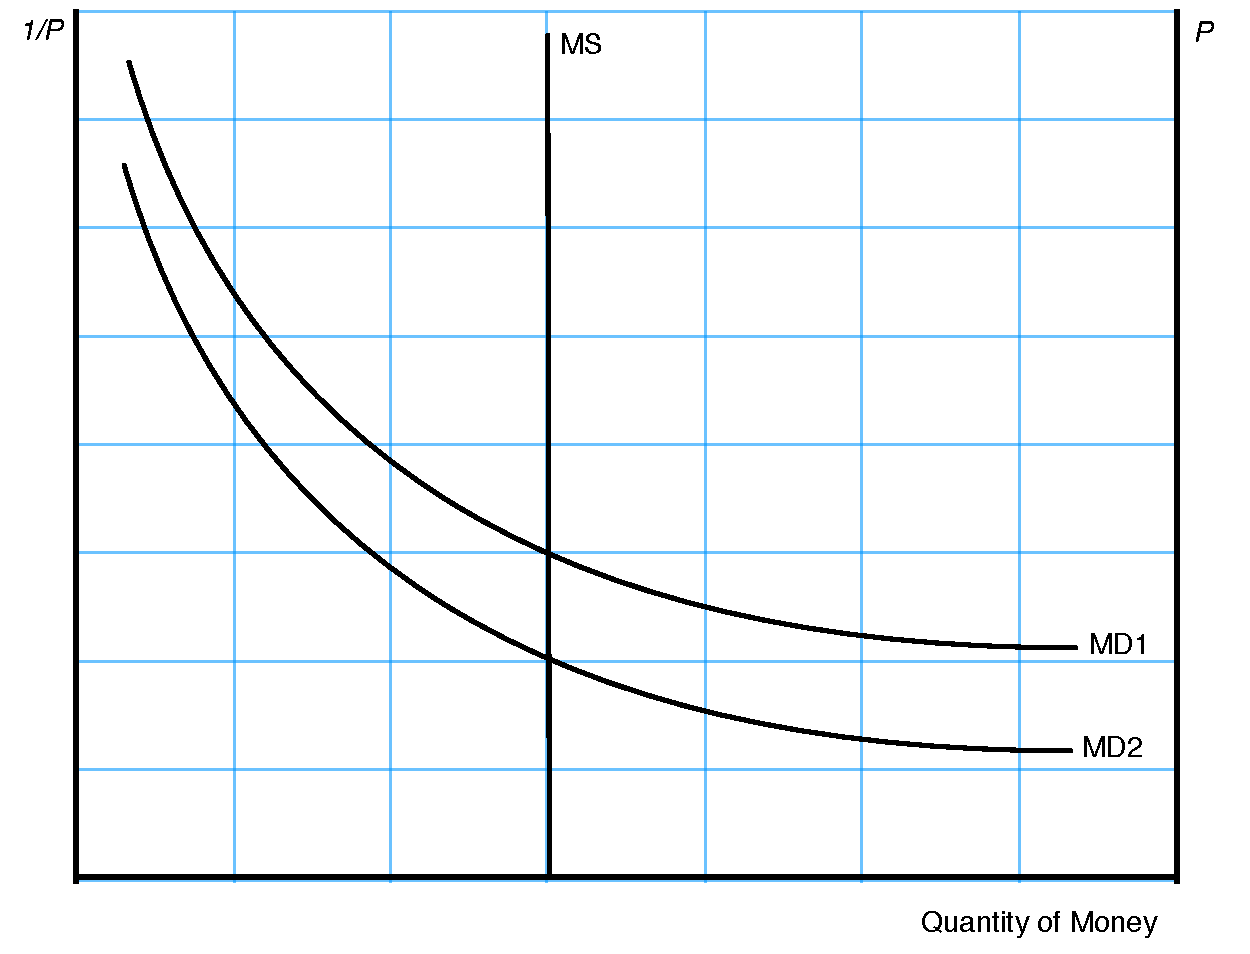
\includegraphics[scale=.40]{Final_MC8.pdf}
		\caption{The Money Market}
		\label{MC8}
	\end{figure}
	

	
	If the demand for money shifts from MD1 to MD2, then we can say that 
	
	\begin{choices}
		\choice the value of money will increase, while the price level will decrease.
		\choice the value of money and the price level will both increase.
		\CorrectChoice the value of money will decrease, while the price level will increase.
		\choice the value of money and the price level will both decrease.
	\end{choices}
	
	\begin{solution}
		A decrease in money demand will decrease the value of money and increase the price level (y-axis on the right is inverted).
	\end{solution}
	

	\question Unexpected deflation will
	
	\begin{choices}
		\choice lower the real value of debts and redistribute wealth from lenders to borrowers.
		\choice lower the real value of debts and redistribute wealth from borrowers to lenders.
		\choice raise the real value of debts and redistribute wealth from lenders to borrowers.
		\CorrectChoice raise the real value of debts and redistribute wealth from borrowers to lenders.
	\end{choices}
	
	\begin{solution}
		Unexpected deflation implies that actual inflation is less than expected, which increases the real value of debts and so wealth is transferred from borrowers to lenders.
	\end{solution}
	
\question An example of a real variable is

\begin{choices}
	\choice the nominal interest rate.
	\CorrectChoice the ratio of the value of wages to the price of soda.
	\choice the price of corn.
	\choice the dollar wage.
	\choice none of the above.
\end{choices}


\question Velocity is 

\begin{choices}
	\CorrectChoice the annual rate of turnover of the money supply.
	\choice the annual rate of turnover of output.
	\choice the annual rate of turnover of business inventories.
	\choice impossible to measure.
\end{choices}


\question If actual inflation turns out to be greater than people had expected, then

\begin{choices}
	\choice wealth was redistributed from borrowers to lenders.
	\CorrectChoice wealth was redistributed from lenders to borrowers.
	\choice no redistribution occurred.
	\choice the real interest rate is unaffected.
\end{choices}

\question If the real interest rate is 4\%, the inflation rate is 6\%, and the tax rate is 20\%, what is the after-tax real interest rate?

\begin{choices}
	\choice 1\%
	\CorrectChoice 2\%
	\choice 3\%
	\choice 4\%
	\choice 5\%
\end{choices}

\question Which of the following is true about a situation where real incomes are rising at 3\% per year?

\begin{choices}
	\choice If inflation were 5\%, people should receive raises of about 8\% per year.
	\choice If inflation were 0\%, people should receive raises of about 3\%.
	\choice If money were neutral, an increase in the money supply will not alter the rate of growth of real income.
	\CorrectChoice All of the above are true.
	\choice None of the above are true.
\end{choices}
	
	\question Suppose that this year's money supply is \$500 billion, nominal GDP is \$10 trillion, and the real GDP is \$5 trillion. 
	
	\begin{parts}
		\part What is the price level? What is the velocity of money? 
		\begin{solution}
			$Mv=PY$, where $PY$ = nominal GDP. $P$ = nominal GDP/real GDP = 10,000/5,000 = 2. Velocity = $PY/M$ = 10,000/500 = 20.
		\end{solution}
		\part Suppose that velocity is constant and the economy's output of goods and services rises by 5\% each year. What will happen to nominal GDP and the price level next year if the Fed keeps the money supply constant?
		\begin{solution}
			$\vec{M} + \vec{v} = \vec{Y} + \pi$. $\vec{v} = 0$, $\vec{Y} = 5\%$. If $\vec{M} = 0$, 0\% + 0\% = 5\% + $\pi \Rightarrow \pi = -5\%$. Prices will decrease by 5\% and nominal GDP will be unchanged.
		\end{solution}
		\part What money supply should the Fed set next year if it wants to keep the price level stable? 
		\begin{solution}
			$\pi^* = 0\% \Rightarrow \vec{M}^* + 0\% = 5\% + 0\% \Rightarrow \vec{M}^* = 5\%$. $MS_1 = 500(1.05) = 525$B.
		\end{solution}
		\part What money supply should the Fed set next year if it wants an inflation of 10\%?
		\begin{solution}
			$\pi^* = 10\% \Rightarrow \vec{M}^* + 0\% = 5\% + 10\% \Rightarrow \vec{M}^* = 15\%$. $MS_1 = 500(1.15) = 575$B.
		\end{solution}
	\end{parts}
	
\end{questions}


	
	\subsection*{AS-AD Model}

\begin{questions}


\question When the economy goes into a recession, real GDP \blank and unemployment \\ \blank.

\begin{choices}
	\choice rises; rises
	\choice rises; falls
	\CorrectChoice falls; rises
	\choice falls; falls
\end{choices}

\newpage

\question A change in the expected price level shifts 

\begin{choices}
	\choice the AD curve.
	\CorrectChoice the short-run AS curve, but not the long-run AS curve.
	\choice the long-run AS curve, but not the short-run AS curve. 
	\choice both the short-run and the long-run AS curve.
\end{choices}

\begin{solution}
	The SRAS curve is determined by $\pi^e$, while the LRAS curve is determined by the natural growth rate.
\end{solution}

\question An increase in the AD for goods and services has a larger impact on output  \blank  and a larger impact on the price level \blank.

\begin{choices}
	\CorrectChoice in the short run; in the long run
	\choice in the long run; in the short run
	\choice in the short run; also in the short run
	\choice in the long run; also in the long run
\end{choices}

\begin{solution}
	An increase in AD will cause output and inflation to rise in the short run. In the long run, inflation will increase further, but output will return to its natural growth rate.
\end{solution}

\question If inflation is greater than expected inflation, 

\begin{choices}
	\CorrectChoice firms' profits will increase.
	\choice money growth will cause the aggregate demand curve to shift.
	\choice firms' profits will decrease.
	\choice there will be no change in real GDP growth in the short run.
\end{choices}


\question Sticky wages and prices 

\begin{choices}
	\choice reduce the impact of negative shocks.
	\CorrectChoice increase the impact of positive shocks.
	\choice have no effect on the impact of negative shocks. 
	\choice offset the impacts of positive shocks.
\end{choices}

\begin{solution}
	Sticky wages and prices increase the impact of both positive and negative shocks. A stickier SRAS curve will have a larger impact on SR real growth in either case.
\end{solution}




\question Which of the following causes the aggregate demand curve to shift left?

\begin{enumerate}[(i)]
	\item Increased taxes
	\item Increased consumer confidence
	\item Increased import growth
\end{enumerate}

\begin{choices}
	\choice i and ii only
	\choice ii and iii only
	\CorrectChoice i and iii only
	\choice i, ii, and iii
\end{choices}



\question Which of the following is an example of a negative shock to an economy?

\begin{choices}
	\choice A decrease in oil prices
	\choice Tax cuts
	\choice New technology
	\CorrectChoice Terrorist attacks
\end{choices}

\newpage

\question Sticky wages and prices

\begin{choices}
	\choice reduce the short-run impact of negative shocks.
	\CorrectChoice increase the short-run impact of positive shocks.
	\choice have no effect on the short-run impact of negative shocks.
	\choice offset the short-run impacts of positive shocks.
\end{choices}

\question A real shock causes 

\begin{choices}
	\choice a shift of the aggregate demand curve.
	\choice a shift of the aggregate demand and the long-run aggregate supply curve.
	\CorrectChoice a shift of the long-run aggregate supply curve.
	\choice a movement along the long-run aggregate supply curve.
	\choice none of the above.
\end{choices}

\question  Beginning in equilibrium in an AS-AD model, an unexpected increase in money supply growth will cause

\begin{choices}
	\CorrectChoice inflation and real growth to increase in the short run.
	\choice inflation to increase and real growth to decrease in the short run.
	\choice inflation to increase and real growth to remain unchanged in the short run.
	\choice inflation and real growth to remain unchanged.
\end{choices}

\question If the growth rate of money is 3\% and the growth rate of velocity is 1\%, the growth rate of nominal GDP is 

\begin{choices}
	\CorrectChoice 4\%.
	\choice 1\%
	\choice 0\%.
	\choice 2\%.
\end{choices}

\question In the AS-AD model, changes in the growth rate of C, I, G, and NX are reflected in changes in 

\begin{choices}
	\choice money supply.
	\CorrectChoice money velocity.
	\choice price levels.
	\choice all of the above.
\end{choices}

\question Other things held constant, an increase in the velocity of money will cause the aggregate demand to 

\begin{choices}
	\CorrectChoice shift right.
	\choice shift left.
	\choice not shift at all.
	\choice shift randomly.
\end{choices}

\newpage

\question Which of the following shocks could shift the long-run aggregate supply curve?

\begin{choices}
	\choice A productivity shock.
	\choice A negative supply shock.
	\choice A real shock.
	\CorrectChoice All of the above.
\end{choices}

\question Use Figure \ref{fig2} to answer the questions that follow. Assume that firms are changing the price of final goods at the same rate as inflation.


\begin{figure}[H]
	\centering
	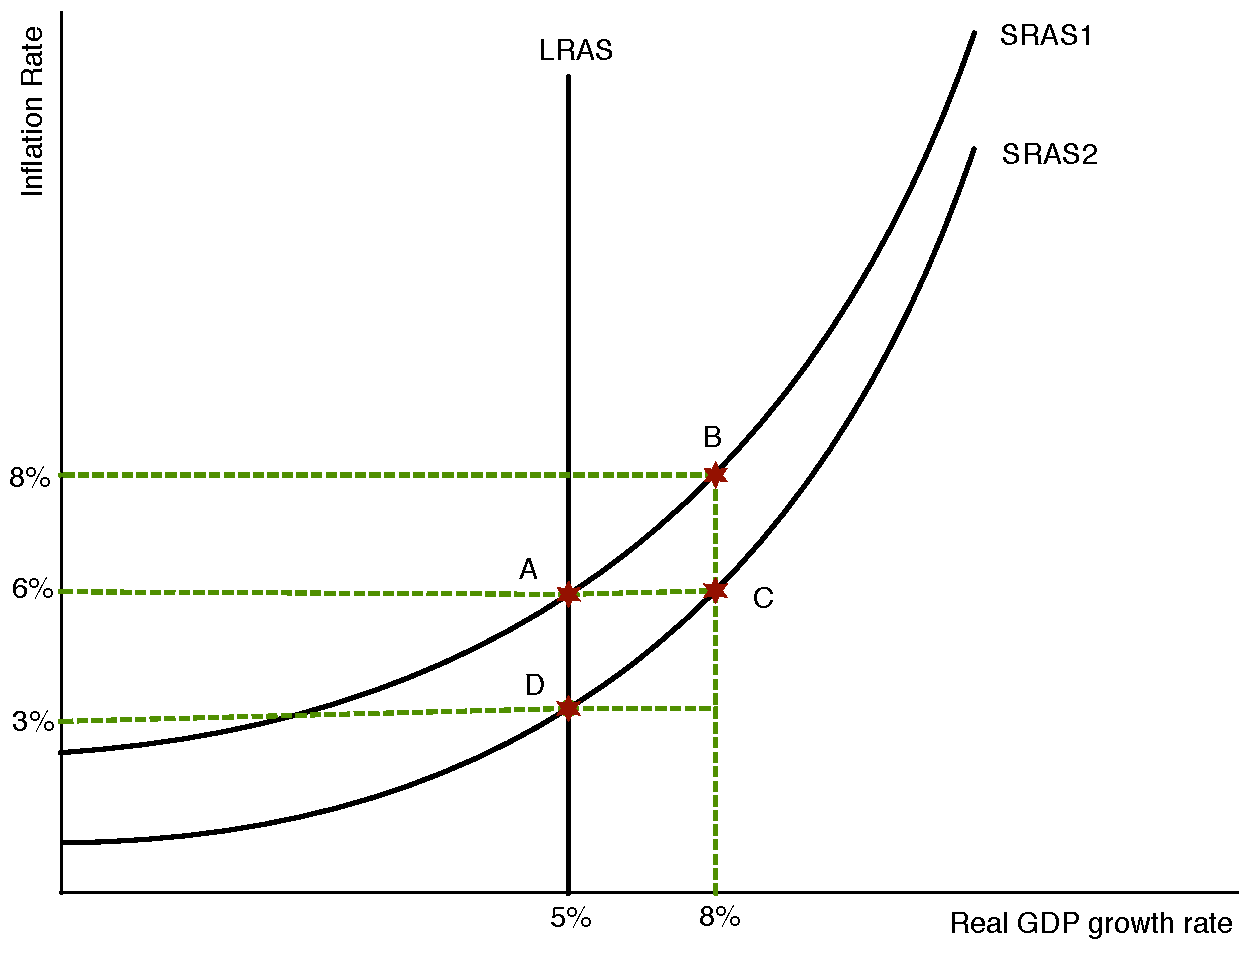
\includegraphics[scale=.45]{hw8_plot1.pdf}
	\caption{SRAS}
	\label{fig2}
\end{figure}

\begin{parts}
	\part If nominal wages are growing at 3\% annually, then at point D how fast are real wages growing? 
	\begin{solution}
		At point D, $\pi = 3\%$. $\%\Delta \text{real wages} = \%\Delta\text{nom. wages} - \pi = 3\% - 3\% = 0\%$.
	\end{solution}
	\part If nominal wages are growing at 3\% annually, then at point C how fast are real wages growing? 
	\begin{solution}
		At point C, $\pi = 6\%$. $\%\Delta \text{real wages} = 3\% - 6\% = -3\%$.
	\end{solution}
	
	\part If nominal wages are growing at a constant rate, what happens to firm profits between points D and C? How will the change in profits affect the growth rate of output?
	
	\begin{solution}
		Between points D and C, firm profits are increasing because expected inflation is less than actual inflation. Prices are rising faster than wages, and so firm profits grow. The growth rate of output will increase to 8\%.
	\end{solution}
	\part Assume we are at point C, and workers are at the point where they can renegotiate wages. In order to maintain the same standard of living that they had at point D, what wage growth rate will they negotiate? 
	\begin{solution}
		At C, $\pi = 6\%$ and so workers will demand nominal wage growth of 6\% in order to return to real wage growth of $0\%$.
	\end{solution}
	\part Will the economy remain at point C? Why or why not? If the point does change, what will the new point be? 
	\begin{solution}
		No. As $\pi^e$ increases, the SRAS curve will shift up until $\pi^e = \pi$ at point A.
	\end{solution}
\end{parts}



\end{questions}

\newpage

\subsection*{Monetary \& Fiscal Policy}

\begin{questions}
	
	\question Imagine that a government starts out with a budget surplus. If in the next period the government temporarily runs a budget deficit, what would you expect to happen to aggregate demand?
	
	\begin{choices}
		\CorrectChoice AD would increase.
		\choice AD would lie at the natural growth of output.
		\choice AD would be unchanged.
		\choice AD would decrease. 
	\end{choices}
	
	\begin{solution}
		A budget deficit would come about because (i) G increased, (ii) taxes decreased, or both. Either way, spending increases and so AD increases.
	\end{solution}
	
	
	\question If the central bank wants to expand aggregate demand, it can \blank the money supply, which would \blank the interest rate.
	
	\begin{choices}
		\choice increase; increase
		\CorrectChoice increase; decrease
		\choice decrease; increase
		\choice decrease; decrease
	\end{choices}
	
	\begin{solution}
		The Fed increases the money supply through open market purchases (buying bonds). Increased demand for bonds raises their price, which in turn decreases the interest rate on those bonds.
	\end{solution}
	

	\question Which of the following is an example of an automatic stabilizer? When the economy goes into a recession,
	
	\begin{choices}
		\CorrectChoice more people become eligible for unemployment insurance benefits.
		\choice stock prices decline, particularly for firms in cyclical industries.
		\choice Congress begins hearings about a possible stimulus package.
		\choice the Fed changes its target for the federal funds rate.
	\end{choices}
	
	
	
	\question When consumers are very reluctant to spend in a recessionary environment, the government's most effective strategy is to 
	
	\begin{choices}
		\CorrectChoice increase spending through bond financing.
		\choice decrease income taxes.
		\choice decrease corporate taxes.
		\choice do nothing - the economy will self-correct in the short run.
	\end{choices}
	
	\begin{solution}
		Government spending is most effective if consumer's are reluctant to spend. Decreasing taxes may not spur spending if most individuals choose to save their extra income.
	\end{solution}
	
\item If the government wants to contract aggregate demand, it can \blank government purchases or \blank taxes.

\begin{choices}
	\choice increase; increase
	\choice increase; decrease
	\CorrectChoice decrease; increase
	\choice decrease; decrease 
\end{choices}

\begin{solution}
	The government can contract AD by either decreasing their own spending or raising taxes.
\end{solution}

\newpage

\question Suppose that a permanent decrease in investment spending causes a recession. If the Fed wishes to counteract this change in aggregate demand in order to get the economy back to its initial real GDP growth rate, it could

\begin{choices}
	\choice sell bonds.
	\choice increase the interest rate on reserves.
	\CorrectChoice lower the discount rate. 
	\choice increase reserve requirements.
	\choice None of the above achieves this goal.
\end{choices}


	
\question Consider Figure \ref{fig1}.


\begin{figure}[H]
	\centering
	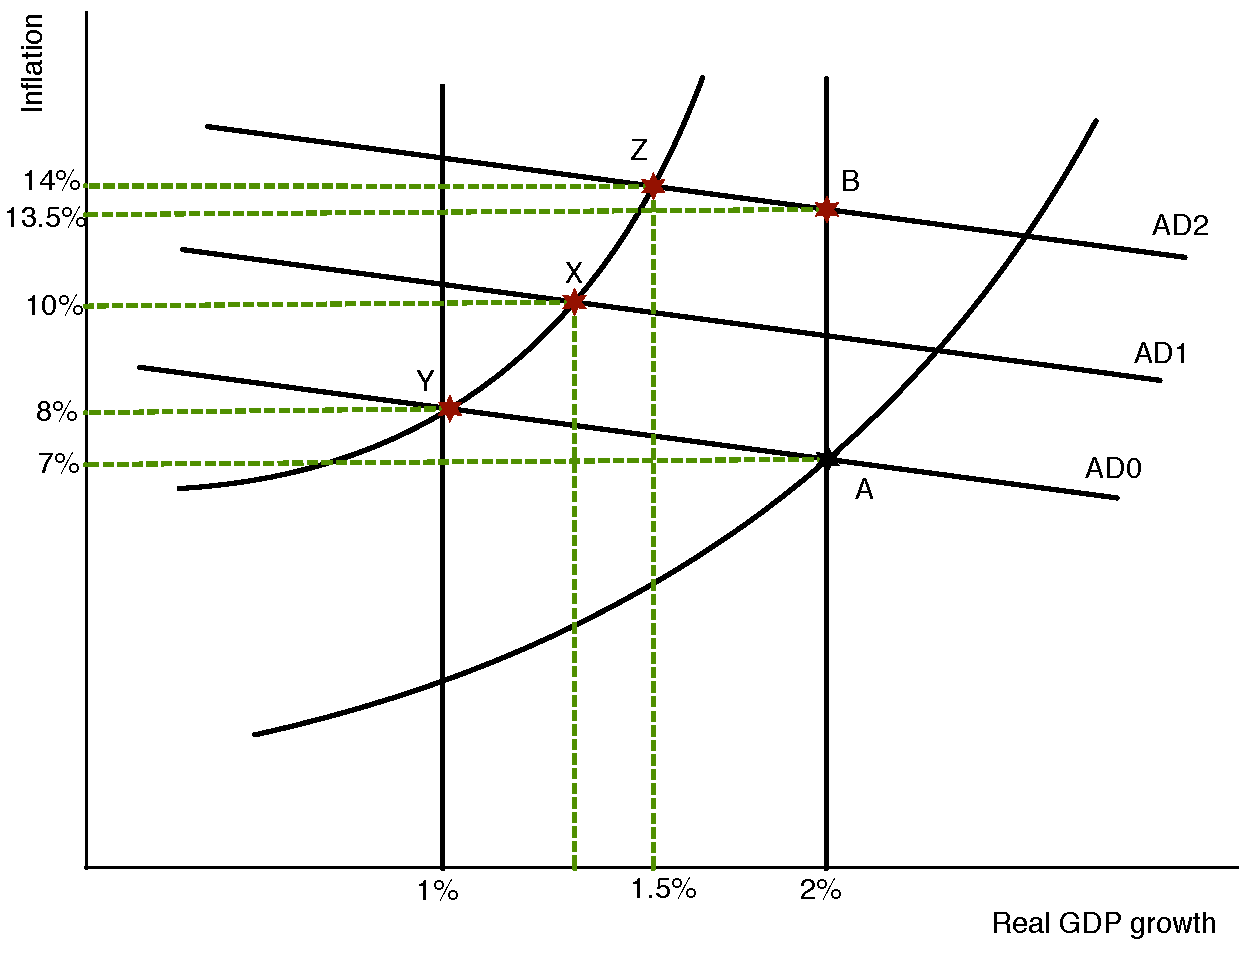
\includegraphics[scale=.45]{ec2_plot1.pdf}
	\caption{Real Shock}
	\label{fig1}
\end{figure}

If after a real shock the economy is operating at point $Y$, then, in the absence of crowding out, fiscal policy that shifted $AD0$ to $AD2$ would move the economy to point

\begin{choices}
	\choice $A$
	\choice $B$
	\CorrectChoice $Z$
	\choice $X$
\end{choices}

\begin{solution}
	Real shock moved LRAS curve from $g=2\%$ to $g=1\%$. Long-run Eq at $AD0$ is $Y$. If AD shifts to $AD2$, economy would be where $AD2$ and the new SRAS curve intersect at point $Z$.
\end{solution}


\question Which of the following poses a limit to fiscal policy?

\begin{choices}
	\choice Crowding out
	\choice Size of government expenditures.
	\choice Timing lags.
	\CorrectChoice All of the above.
\end{choices}

\question 


\uplevel{For questions \ref{q14}-\ref{q15}, refer to Figure \ref{MC14}. Suppose an economy is operating at point $G$ and assume this position came about through a permanent demand side shock.}


\begin{figure}[H]
	\centering
	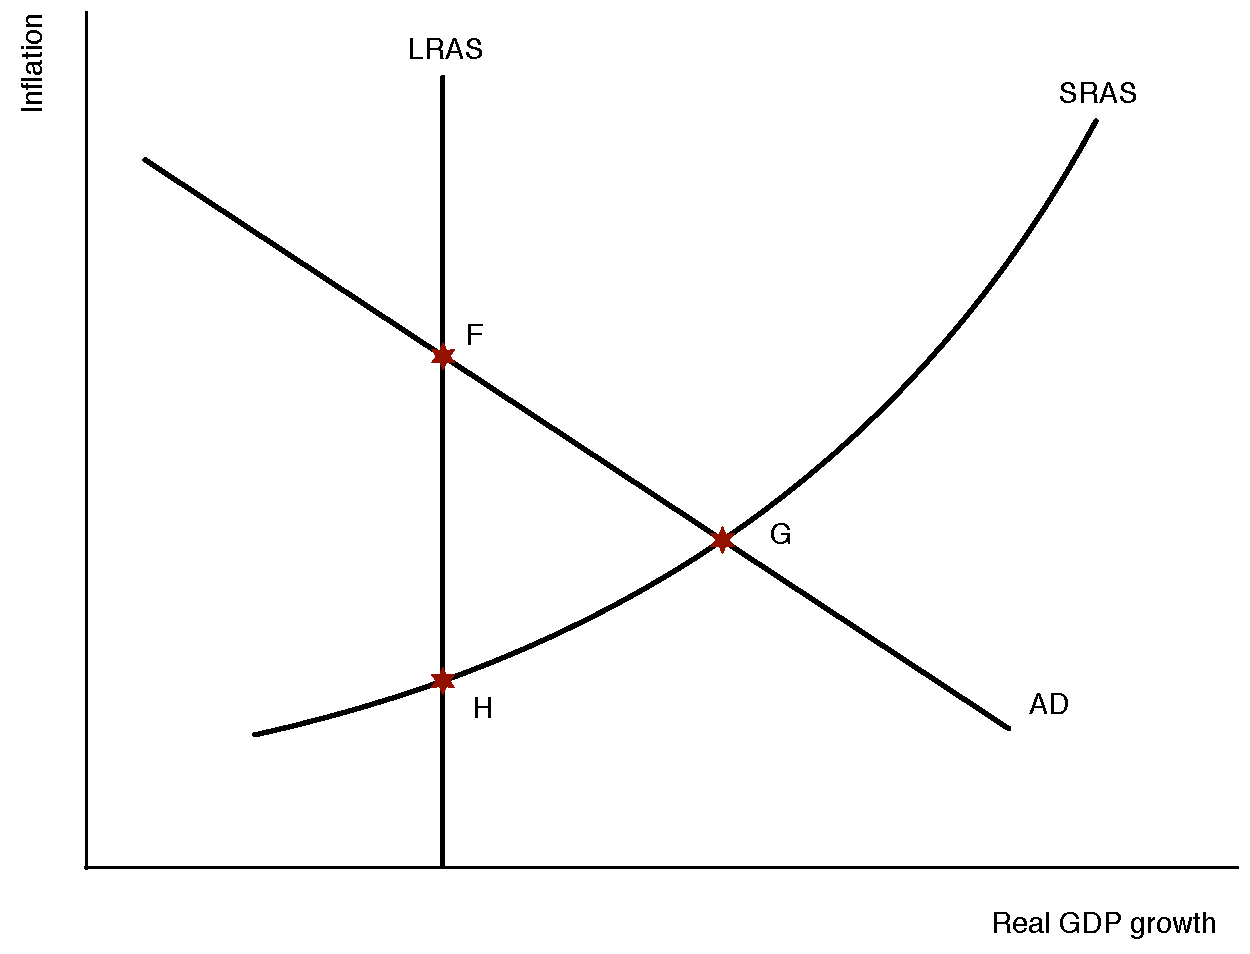
\includegraphics[scale=.38]{Final_MC14.pdf}
	\caption{AS-AD Model}
	\label{MC14}
\end{figure}

\question \label{q14} At point $G$, actual inflation is \blank than expected inflation, and real GDP growth is \blank the natural rate.

\begin{choices}
	\choice less; above 
	\choice less; below
	\choice greater; below
	\CorrectChoice greater; above
\end{choices}

\question \label{q15} In the absence of monetary or fiscal policy, as the economy transitions to its long-run equilibrium,

\begin{choices}
	\choice expected inflation will increase and real GDP growth will increase.
	\choice expected inflation will decrease and real GDP growth will increase.
	\CorrectChoice expected inflation will increase and real GDP growth will decrease.
	\choice expected inflation will decrease and real GDP growth will decrease.
\end{choices}


\question Expansionary fiscal policy can reduce real growth if the increase in government spending

\begin{choices}
	\choice causes a large enough increase in private spending.
	\CorrectChoice causes a large enough decrease in private spending.
	\choice is believed to be temporary.
	\choice is believed to be permanent.
\end{choices}

\question Fiscal policies that help an economy in a recession without additional actions by policy makers are called

\begin{choices}
	\choice consumption smoothers.
	\choice Ricardian equalizers.
	\CorrectChoice automatic equalizers.
	\choice all of the above.
\end{choices}

\question When expansionary fiscal policy increases income and consumer spending, the subsequent increase in aggregate demand is called the \blank effect.

\begin{choices}
	\choice expansionary
	\choice secondary
	\CorrectChoice multiplier
	\choice None of the above
\end{choices}


		\question Suppose that an economy has a natural growth rate of 2\%. Moreover, the central bank in the country has perfect control over the money supply and increases it by 4\% every year. Assume spending is such that the velocity of money is constant over time and that the economy is currently at its long-run equilibrium.
		
		\begin{parts}
			
			\part Draw a clearly labeled dynamic AS-AD diagram that shows the long-run equilibrium point, as well as the economy's current growth rate of real GDP, inflation, and expected inflation. Label this point $E_0$. Be sure to include both the short-run and long-run aggregate supply curves. 
			
			\begin{solution}
				Long-run equilibrium is where AD, LRAS, and SRAS meet. LRAS is at real GDP growth of 2\%. Spending growth = $\vec{M} + \vec{v} = 4\%$ since $\vec{v} = 0\%$ and money growth is 4\%. By the Quantity Theory of Money, $\vec{M} + \vec{v} = \vec{Y} + \pi$. Since $\vec{Y} = 2\%$, it must be that inflation in the long run is 2\%. Finally, $\pi^e = \pi = 2\%$ at the long run equilibrium.
				\begin{figure}[H]
					\centering
					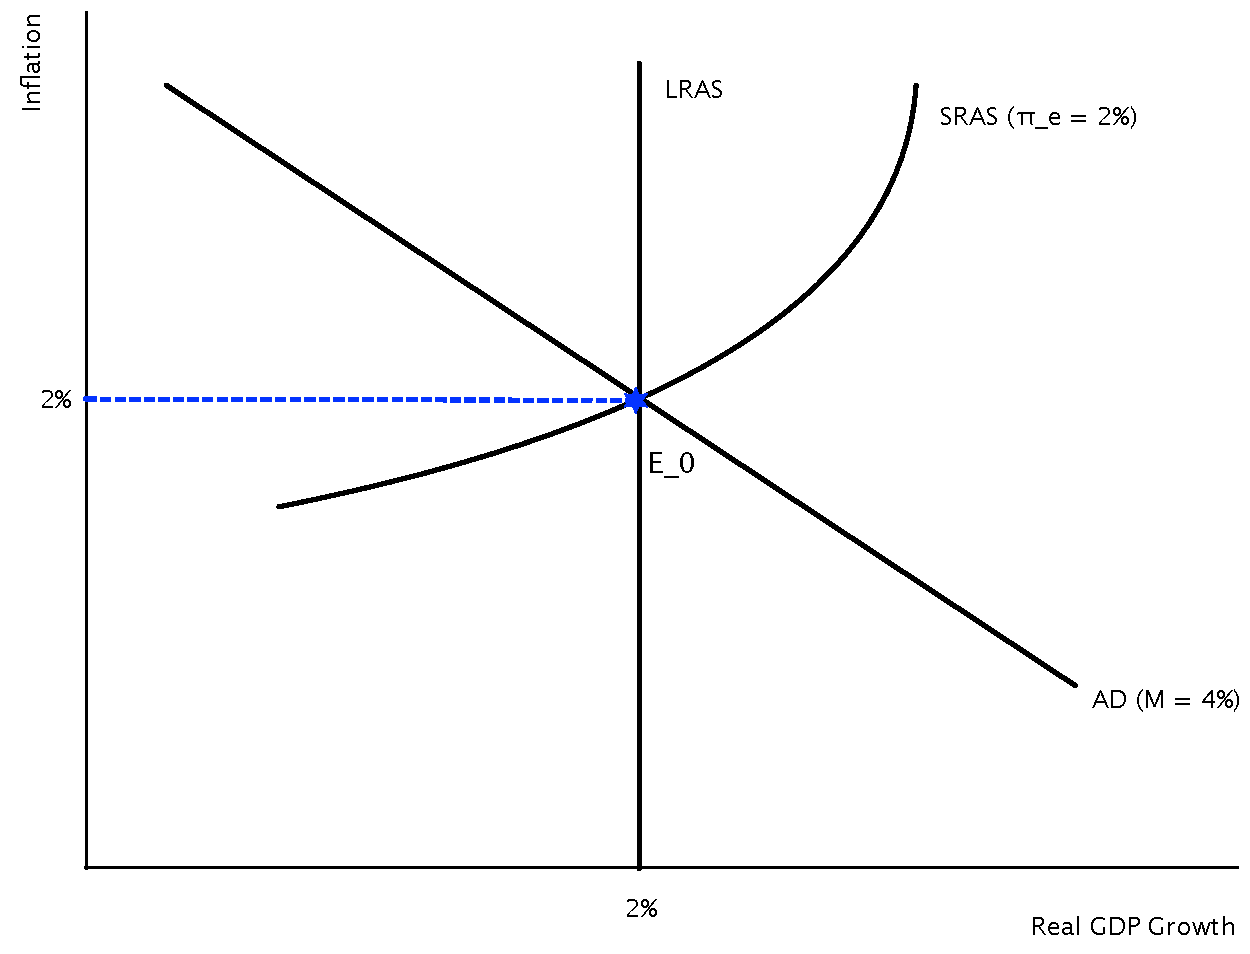
\includegraphics[scale=.4]{hw6_plot1.pdf}
					\caption{AS-AD Model}
				\end{figure}
			\end{solution}
			
			\part Now, suppose that the stock market declines sharply, reducing consumers' wealth. As a result, consumers spend at a rate that is 4\% lower than before. Assume this change is permanent. Does this affect aggregate demand, short-run aggregate supply, or long-run aggregate supply? Explain why. 
			
			\begin{solution}
				This would affect aggregate demand because it would impact consumption spending. Now, $\vec{v} = -4\%$.
			\end{solution}
			
			
			\part Show this change graphically. Assume that neither the central bank nor the federal government enact any policies to counteract this change. Label the short-run equilibrium point $A$ and the long-run equilibrium point $E_1$. What is the inflation rate in the short run if this change in consumer spending caused real GDP growth to decrease to $-1\%$? What will be the long-run real GDP growth rate and inflation rate? 
			
			\begin{solution}
				This decrease in AD is shown in Figure \ref{fig4}. AD shifts left to the AD curve where $\vec{M} + \vec{v} = 4\% + (-4\%) = 0\%$. The short-run point is where the new AD curve and the old SRAS curve meet at point A. If real GDP growth is $-1\%$ at this point, then short-run inflation must be 1\% since spending growth is 0\%. The long-run point $E_1$ is given by where the new AD curve meets the LRAS curve. Long-run growth is the natural rate of 2\%. Since spending growth is 0\%, long-run inflation must be $-2\%$.
				
				
				
				\begin{figure}[H]
					\centering
					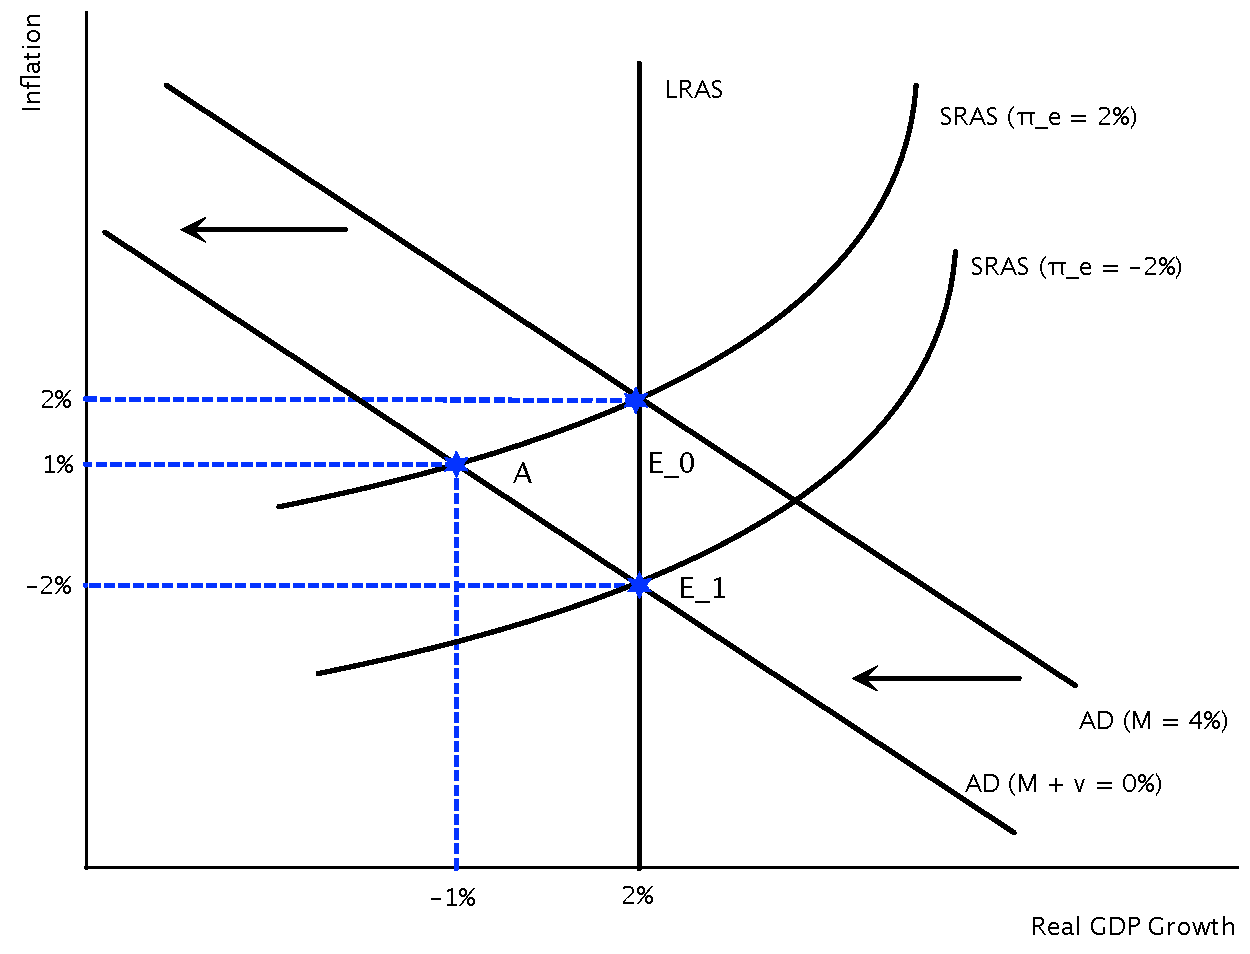
\includegraphics[scale=.4]{hw6_plot2.pdf}
					\caption{Decrease in AD}
					\label{fig4}
				\end{figure}
				
			\end{solution}
			\part Explain why the short-run growth rate of output is different from the long-run growth rate of output. What causes the economy to move from point $A$ to point $E_1$? 
			
			\begin{solution}
				At point A (the short run), actual inflation is less than expected inflation. Thus, firm wages are rising faster than prices and thus firm profits are falling. Due to this, firms will decrease production and in turn real GDP growth will fall. Movement to the long-run point will occur when expected inflation changes to the new long-run inflation rate and the SRAS curve shifts to the right.
			\end{solution}
			
			\part Suppose the central bank decides to intervene while the economy is at point $A$ in order to get the economy back to point $E_0$. Regardless of the policy pursued, show how this policy would be reflected graphically. Specify what the growth rate of the money supply must be in order for this policy to achieve its goal. 
			
			\begin{solution}
				In order to shift the economy back to point $E_0$, the Fed has to increase aggregate demand. To do so, it must return spending growth to 4\%. If $\vec{v} = -4\%$, then the new growth rate of money the Fed must impose is 8\% since $8\% + (-4\%) = 4\%$.
				
				
				\begin{figure}[H]
					\centering
					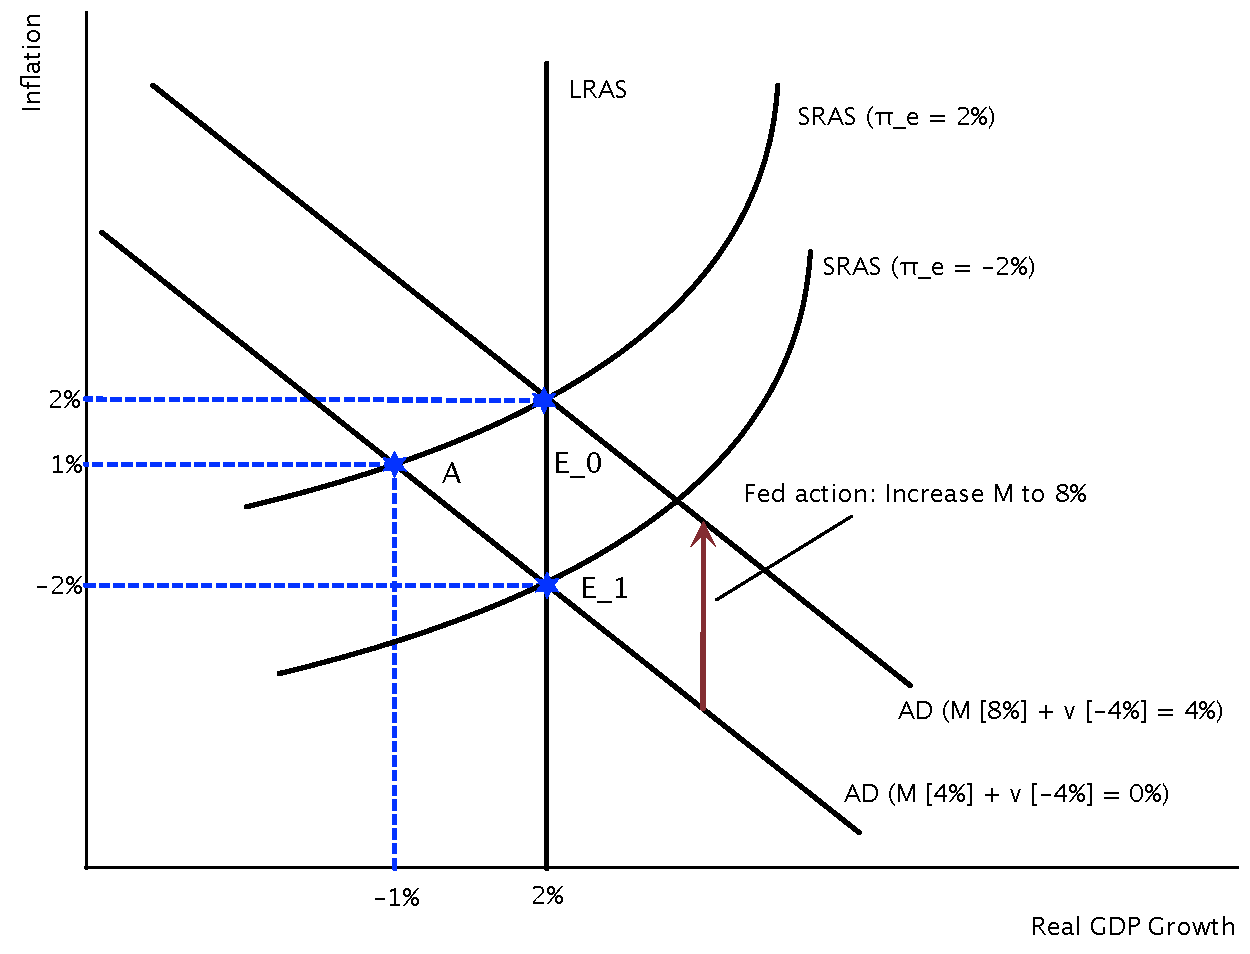
\includegraphics[scale=.4]{hw6_plot3.pdf}
					\caption{Fed Action}
				\end{figure}
				
			\end{solution}
			
		\end{parts}
	
\end{questions}


\end{document}